\documentclass[aspectratio=169]{beamer}

\mode<presentation>
{
  \usetheme{default}
  \usecolortheme{default}
  \usefonttheme{default}
  \setbeamertemplate{navigation symbols}{}
  \setbeamertemplate{caption}[numbered]
  \setbeamertemplate{footline}[frame number]  % or "page number"
  \setbeamercolor{frametitle}{fg=white}
  \setbeamercolor{footline}{fg=black}
} 

\usepackage[english]{babel}
\usepackage[utf8x]{inputenc}
\usepackage{tikz}
\usepackage{courier}
\usepackage{array}
\usepackage{bold-extra}
\usepackage{minted}
\usepackage[thicklines]{cancel}

\xdefinecolor{dianablue}{rgb}{0.18,0.24,0.31}
\xdefinecolor{darkblue}{rgb}{0.1,0.1,0.7}
\xdefinecolor{darkgreen}{rgb}{0,0.5,0}
\xdefinecolor{darkgrey}{rgb}{0.35,0.35,0.35}
\xdefinecolor{darkorange}{rgb}{0.8,0.5,0}
\xdefinecolor{darkred}{rgb}{0.7,0,0}
\definecolor{darkgreen}{rgb}{0,0.6,0}
\definecolor{mauve}{rgb}{0.58,0,0.82}

\title[2018-04-30-paris-oamap]{Object-array mapping and columnar data granularity}
\author{Jim Pivarski}
\institute{Princeton University -- DIANA-HEP}
\date{April 30, 2018}

\begin{document}

\logo{\pgfputat{\pgfxy(0.11, 7.4)}{\pgfbox[right,base]{\tikz{\filldraw[fill=dianablue, draw=none] (0 cm, 0 cm) rectangle (50 cm, 1 cm);}\mbox{\hspace{-8 cm}
\includegraphics[height=1 cm]{princeton-logo-long.png}
\includegraphics[height=1 cm]{diana-hep-logo-long.png}}}}}

\begin{frame}
  \titlepage
\end{frame}

\logo{\pgfputat{\pgfxy(0.11, 7.4)}{\pgfbox[right,base]{\tikz{\filldraw[fill=dianablue, draw=none] (0 cm, 0 cm) rectangle (50 cm, 1 cm);}\mbox{\hspace{-8 cm}
\includegraphics[height=1 cm]{princeton-logo.png}
\includegraphics[height=1 cm]{diana-hep-logo.png}}}}}

% Uncomment these lines for an automatically generated outline.
%\begin{frame}{Outline}
%  \tableofcontents
%\end{frame}

% START START START START START START START START START START START START START

\begin{frame}{Context}
\vspace{0.35 cm}
\begin{columns}[t]
\column{0.4\linewidth}
\underline{High Performance Computing (HPC)}

\vspace{0.15 cm}
\begin{itemize}
\item A lot of focus on data contiguity, CPU cache efficiency, and vectorization.
\item Data structures are often converted to flat arrays or tables, making it easier to reason about such issues.
\end{itemize}

\column{0.56\linewidth}
\begin{uncoverenv}<2->
\underline{High Energy Physics (HEP)}

\vspace{0.15 cm}
\begin{itemize}
\item Data structures are generally:

\begin{center}
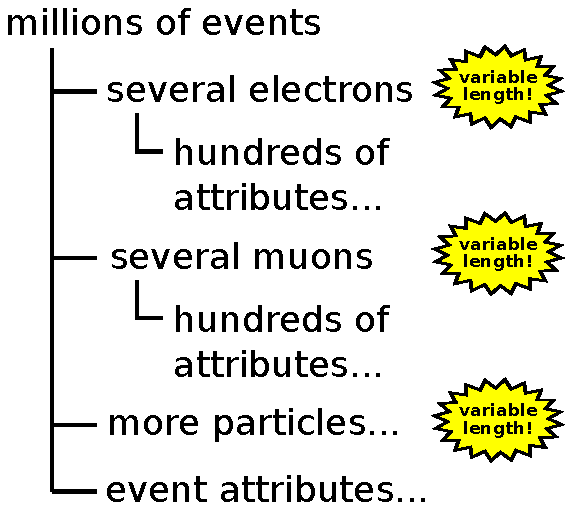
\includegraphics[width=0.7\linewidth]{event-structure.pdf}
\end{center}

\item Analysis code is branchy and pointer-heavy;

``Looks more like string processing!''
\end{itemize}
\end{uncoverenv}
\end{columns}
\end{frame}

\begin{frame}{Context}
\vspace{0.5 cm}
Preparing data for analysis consists of {\it copying} parts of the centrally produced dataset.

\vspace{0.25 cm}
The choice of events to ``skim'' and which attributes to ``slim'' has to be decided before interactive data exploration is possible (timescale of seconds).

\vspace{0.5 cm}
\begin{columns}[c]
\column{0.5\linewidth}
\mbox{ } \hfill 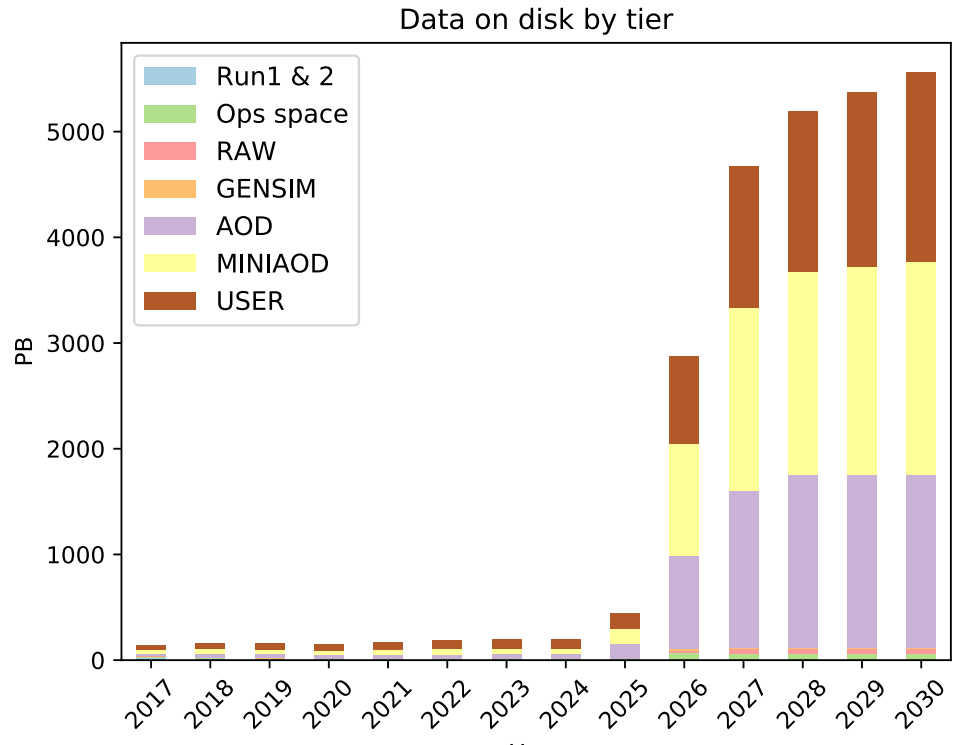
\includegraphics[height=4.5 cm]{cms-data-explosion.png}

\column{0.5\linewidth}

\vspace{0.2 cm}
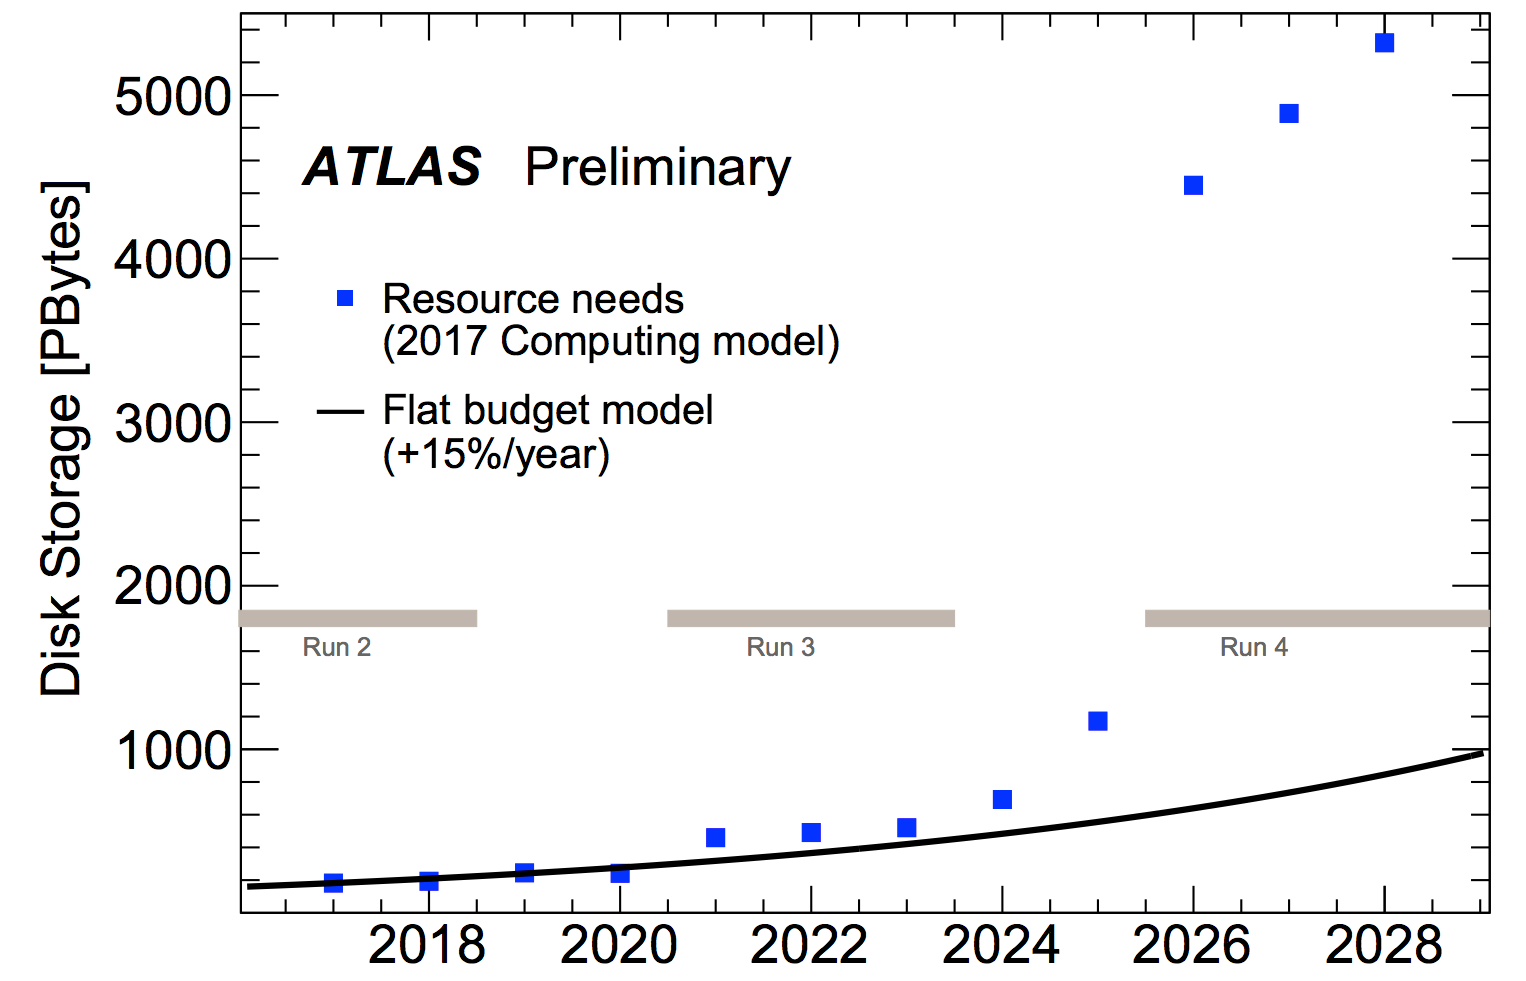
\includegraphics[height=4.4 cm]{atlas-data-explosion.png} \hfill \mbox{ }
\end{columns}
\end{frame}

\end{document}
